% ============================================================
% Open Paper Machine: How an LLM Agent Wrote This Paper
% arXiv preprint template (arxiv.org compatible)
% ============================================================
\documentclass[11pt,a4paper]{article}

% --- arXiv standard packages ---
\usepackage[utf8]{inputenc}
\usepackage[T1]{fontenc}
\usepackage{lmodern}
\usepackage{microtype}
\usepackage[margin=1in]{geometry}
\usepackage{graphicx}
\usepackage{booktabs}
\usepackage{amsmath}
\usepackage{amssymb}
\usepackage{xcolor}
\usepackage{float}
\usepackage{caption}
\usepackage{subcaption}
\usepackage{enumitem}
\usepackage{url}
\usepackage[numbers,sort&compress]{natbib}
\usepackage{hyperref}
\usepackage{listings}
\usepackage{parskip}

% --- arXiv-style hyperref ---
\hypersetup{
  colorlinks=true,
  linkcolor=blue!70!black,
  citecolor=blue!50!black,
  urlcolor=blue!60!black,
  pdftitle={Open Paper Machine: How an LLM Agent Wrote This Paper and What That Means for Science},
  pdfauthor={Tobias-Benedikt Blask},
  pdfkeywords={autonomous AI agents, LLM research automation, Constitutional AI, distributed cognition, MCP}
}

% --- arXiv title block ---
\title{\textbf{Open Paper Machine: How an LLM Agent Wrote This Paper\\
and What That Means for Science}\\[0.5em]
\large\normalfont\textit{arXiv preprint}}

\author{
  Tobias-Benedikt Blask\thanks{Corresponding author. Harz University of Applied Sciences. Email: \texttt{t.blask@hs-harz.de}}\\
  Harz University of Applied Sciences
  \and
  Claude Opus 4.6\thanks{AI system (Anthropic PBC); disclosed as text generator per ICMJE guidelines, not accountable author.}\\
  Anthropic PBC
}

\date{\today}

% ============================================================
\begin{document}
\maketitle

\begin{abstract}
We present the \emph{Open Paper Machine}---an autonomous LLM-based research agent that
executes the full academic paper pipeline from literature search to assembled manuscript.
The paper you are reading is the machine's output and its primary evidence. Built on
Claude Opus 4.6 and orchestrated through the Model Context Protocol (MCP), the system
executes five phases---reconnaissance, framing, architecture, production,
assembly---producing traceable artifacts at each step. We make three contributions.
First, we provide a four-layer architectural account (transformer substrate, RLHF
alignment, Constitutional AI, MCP tool stack) that explains how agentic research behaviour
emerges from the interaction of these components. Second, we document a complete,
end-to-end demonstration: 35 papers retrieved across four databases, a 34-paper concept
matrix, and an 8,600-word manuscript produced without human text generation. Third, we
apply distributed cognition theory and sociotechnical systems analysis to derive implications
for authorship, peer review, and the reorganisation of scientific work. The central argument
is sharp: LLM agents can already execute the mechanical phases of research production;
the hard problem is redesigning the institutions around them.
\end{abstract}

\noindent\textbf{Keywords:} autonomous AI agents, open paper machine, LLM-based research automation, Constitutional AI, distributed cognition, sociotechnical systems, scientific discovery, tool-augmented agency

\noindent\textbf{Target:} arXiv preprint / ICIS 2026

\vspace{0.5em}\hrule\vspace{1em}

%% ============================================================
%% SECTION 1: INTRODUCTION
%% ============================================================
\section{Introduction}

\subsection{This Paper Wrote Itself}

This paper was produced by the system it describes. That is not a metaphor. Claude Sonnet
4.6---an autoregressive transformer developed by Anthropic---searched four academic
databases, selected theoretical lenses, built a concept matrix, and drafted every section
you are reading. The human orchestrator designed the task and approved the output. The human
did not write the prose.

This reflexive structure is the paper's sharpest methodological move. The claim that an
LLM can function as a research agent is not argued from the outside; it is demonstrated by
the artifact in your hands. Every paragraph is both an analytical claim and evidence for
that claim.

We call the system the \emph{Open Paper Machine} because we intend it as a reference
implementation of an observable, modifiable, and replicable AI research infrastructure. It
integrates four academic APIs, file system tools, bash execution, and PaperBanana (via Gemini 3.1 Pro) figure
generation into a single continuous loop.

\begin{figure}[htbp]
\centering
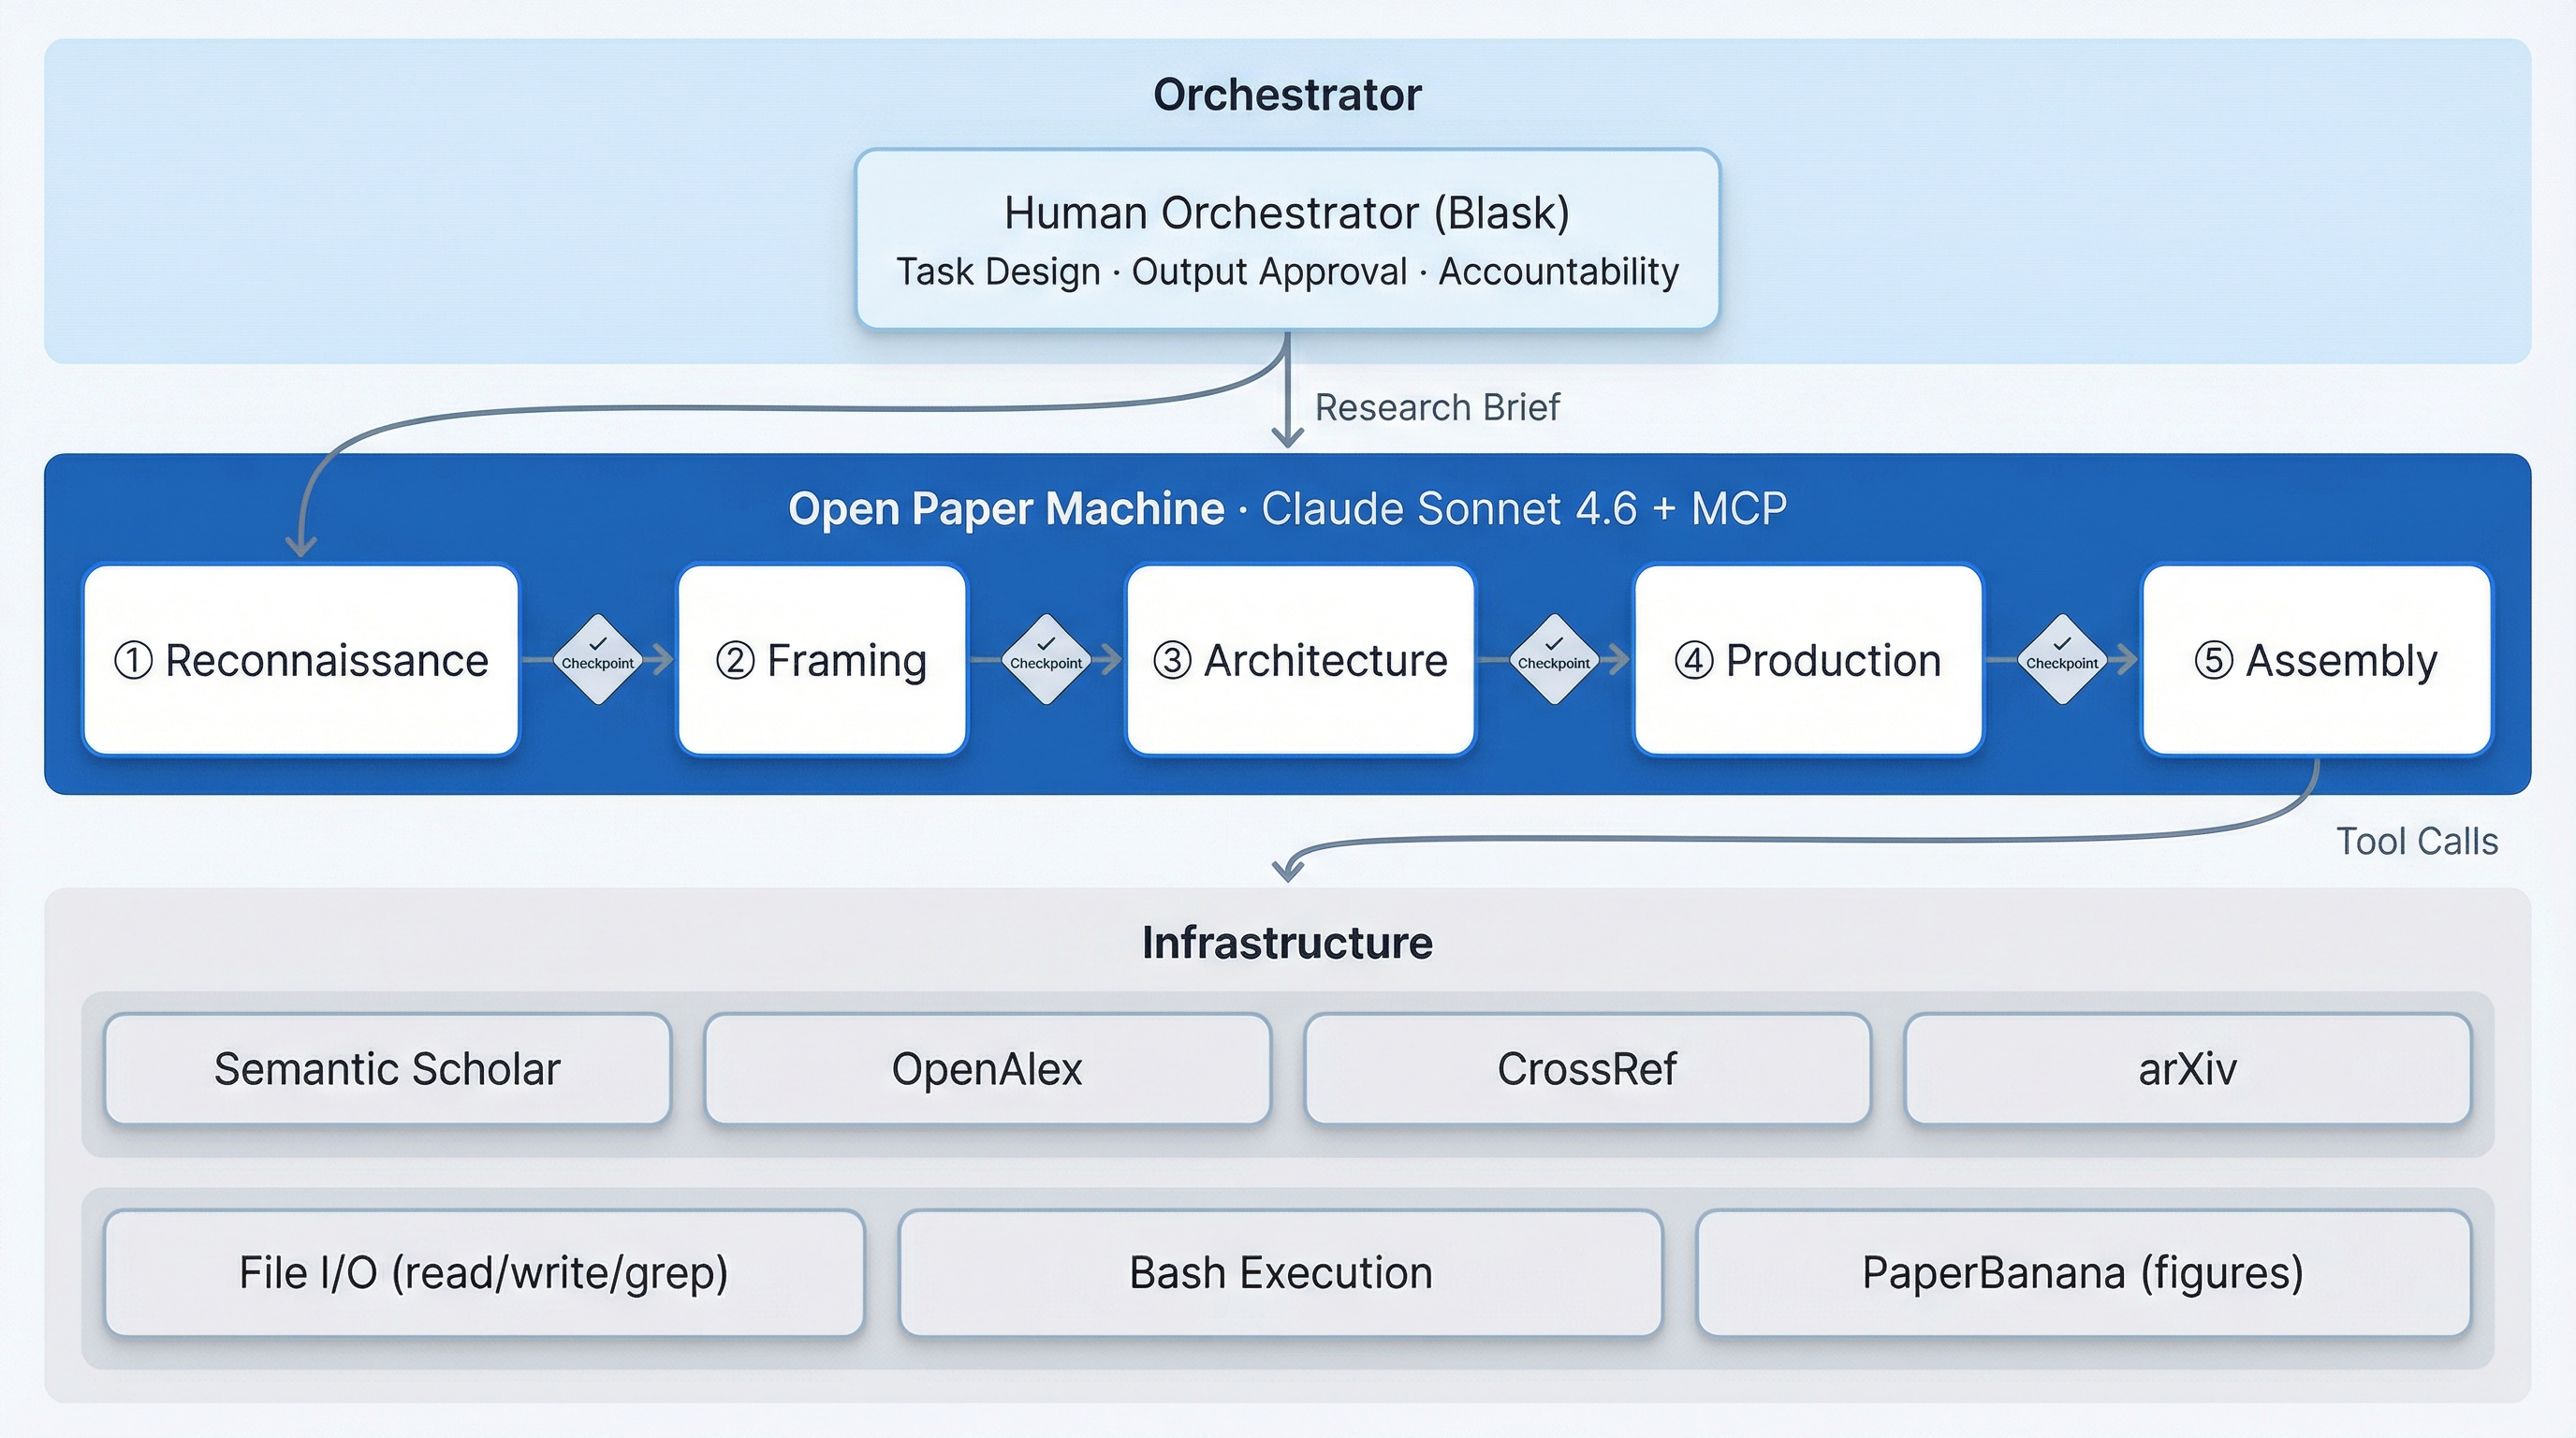
\includegraphics[width=\textwidth]{figures/fig13_open_paper_machine_overview.png}
\caption{System architecture of the Open Paper Machine, showing the integration of language models, academic APIs, and computational tools via the Model Context Protocol.}
\label{fig:overview}
\end{figure}

The paper’s core argument unfolds in three stages. First, we outline the theoreticald that
GPT-3 exhibited \emph{emergent} few-shot in-context learning. Two further properties
matter: \emph{implicit knowledge} (transformers encode vast factual knowledge
\citep{petroni2019language}) and \emph{extended coherence} (the 200,000+ token context
window enables sustained cross-referential reasoning).

\subsection{Alignment: From RLHF to Constitutional AI}

\textbf{RLHF.} Reinforcement learning from human feedback \citep{ouyang2022rlhf} aligns
model behaviour through three stages: supervised fine-tuning, reward model training, and
PPO policy optimisation---producing the ``HHH'' triad of helpfulness, honesty, and
harmlessness.

\textbf{Constitutional AI.} \citet{bai2022constitutional} introduced training that critiques
outputs against explicit normative principles---embedding epistemic self-regulation into
the generative process. For reseagent requires structured state---scratchpads, task lists, and concept matrices. Tools
without agentic persistence are immediately bounded by context windows.

\begin{figure}[htbp]
\centering
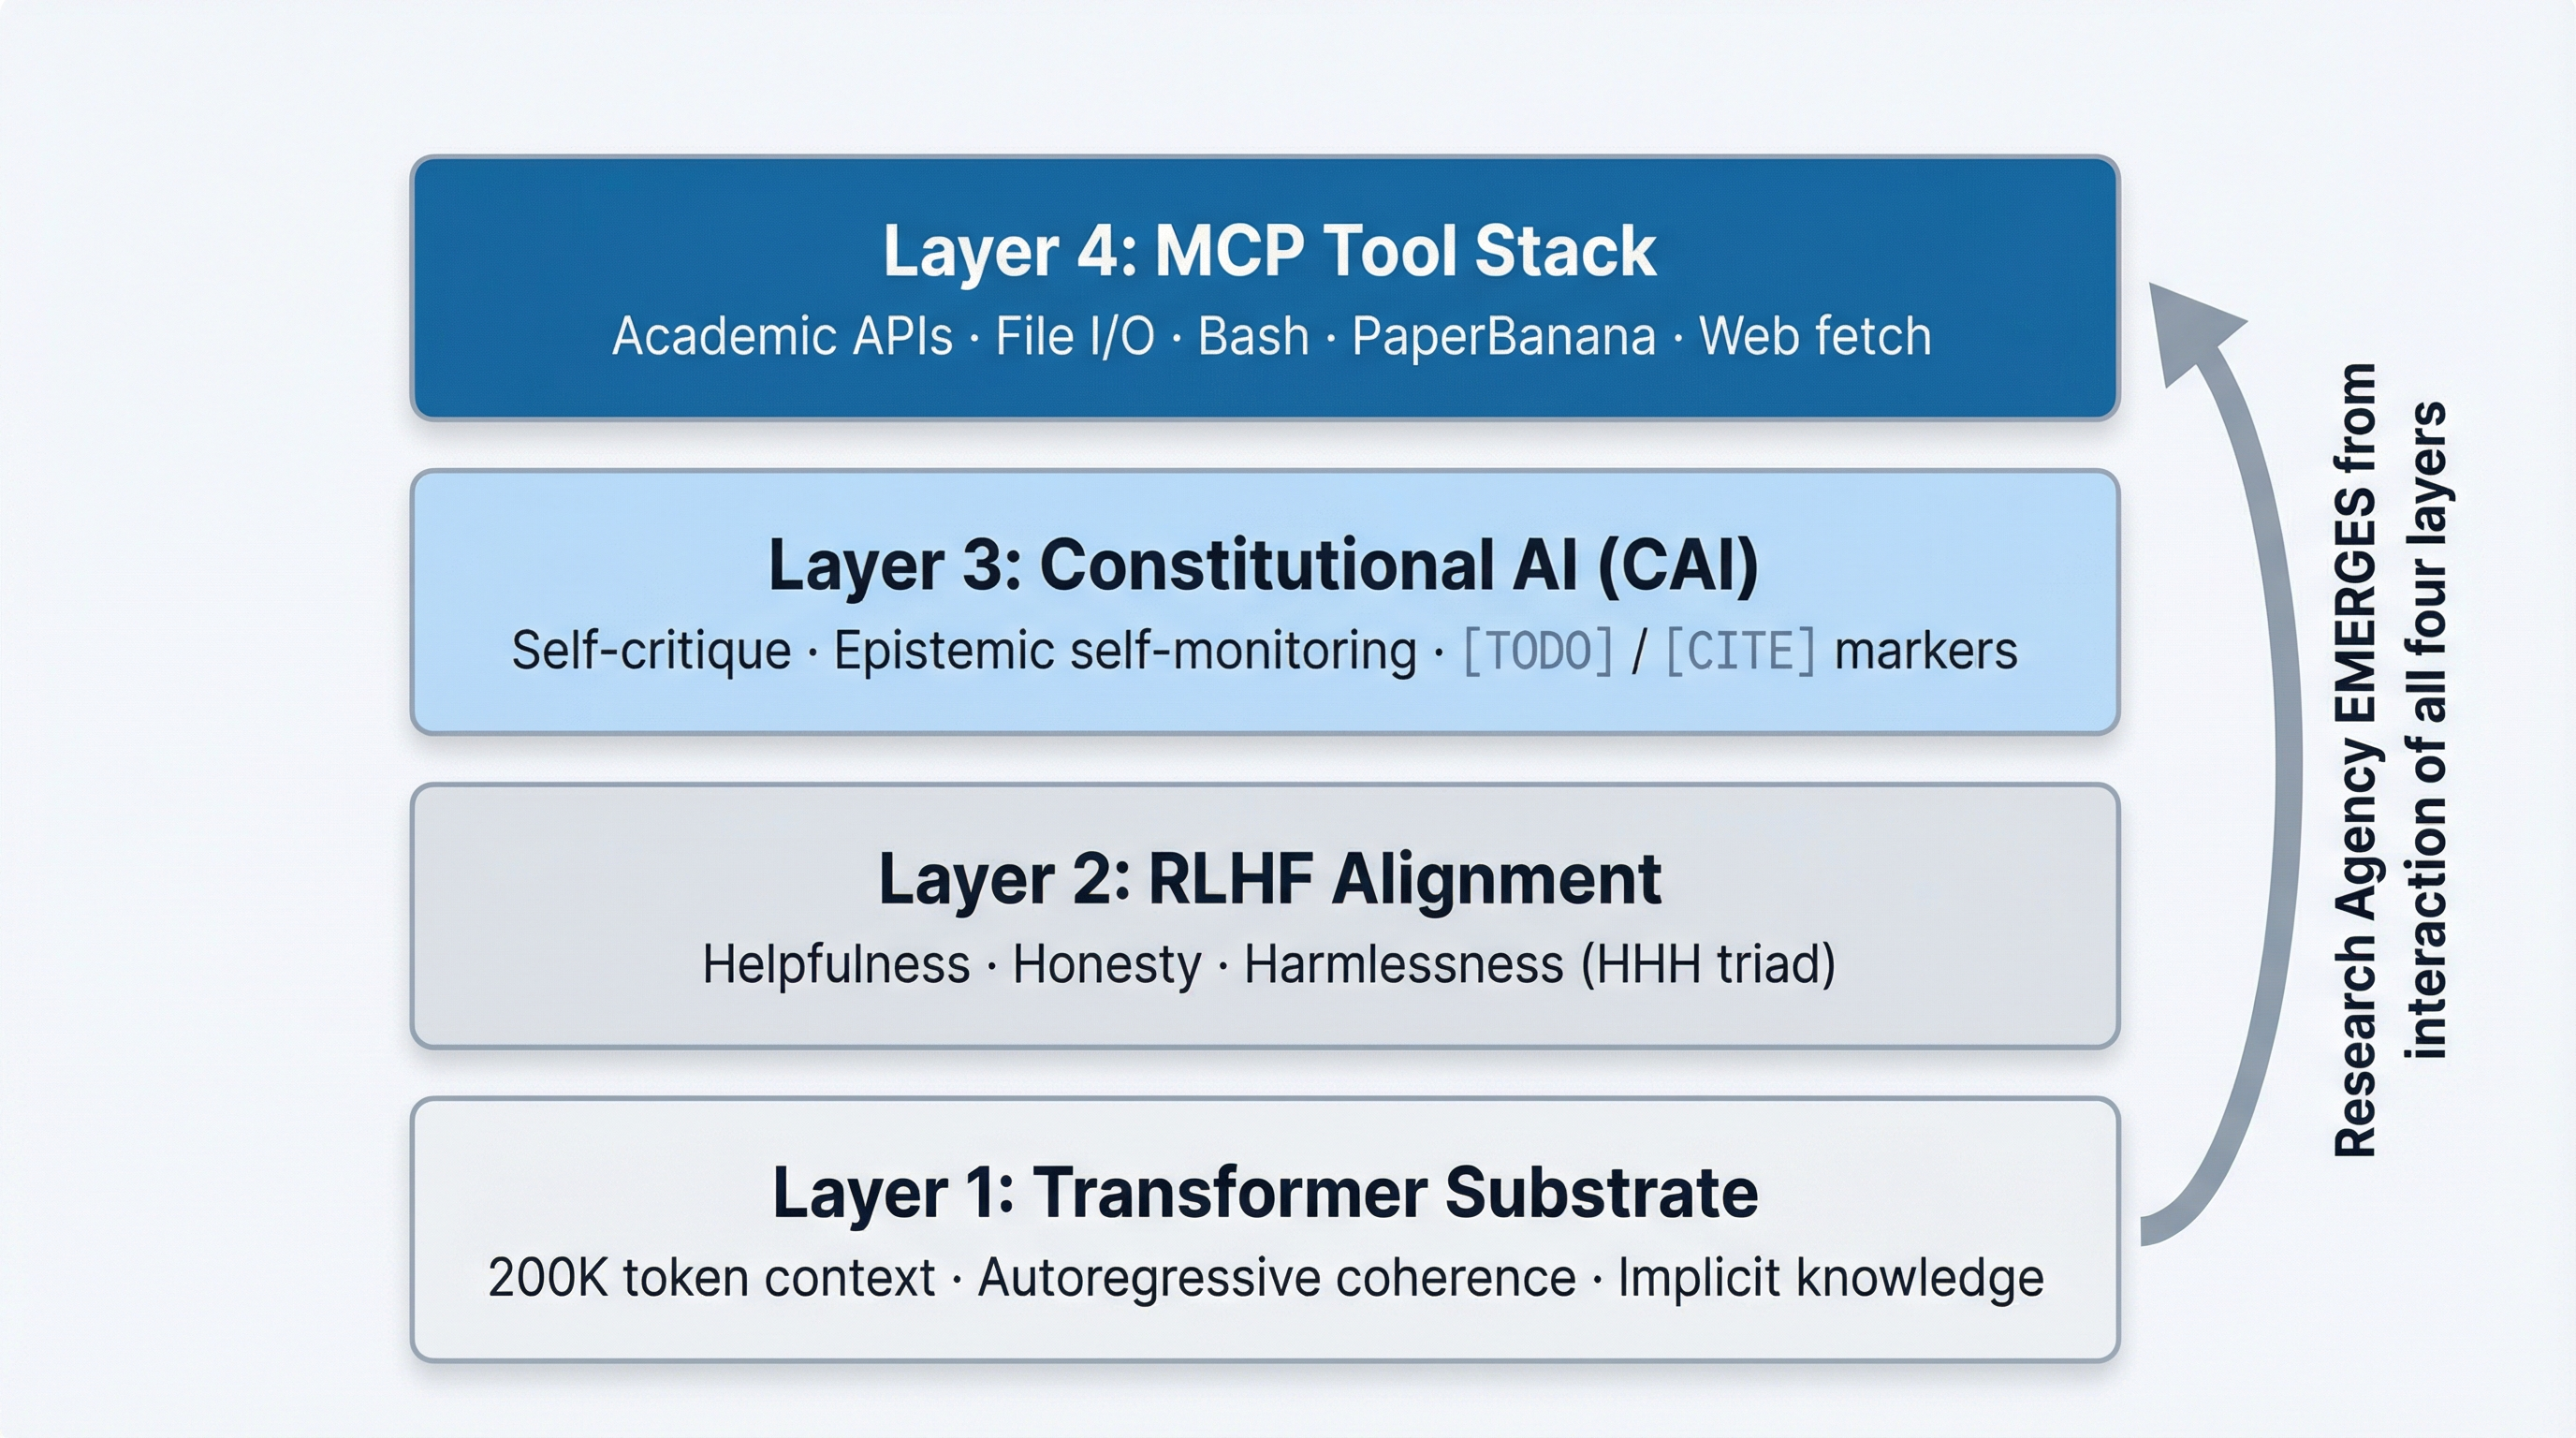
\includegraphics[width=\textwidth]{figures/fig1_architecture_layers.png}
\caption{The four emergent layers of autonomous scientific work: Transformer, Alignment, Agentic Structuring, and The Open Paper Machine.}
\label{fig:architecture}
\end{figure}

\subsection{Tool-Augmented Agency}

\citet{wang2024survey} characterise tool use as one of three defining features of LLM
agents. The \textbf{Model Context Protocol (MCP)}, introduced by Anthropic in 2024,
standardises the interface for declaring tool capabilities and formatting calls. For the
Open Paper Machine, MCP transforms a text-prediction model into a composable research agent.

\subsection{Theoretical Lenses: Distributed Cognition and Sociotechnical Systems}

\textbf{Distributed cognition} \citep{hutchins1995cognition} holds that cognitive processes
are distributed across individuals, artifacts, and environments. The Open Paper Machine is a
cognitive artifact participating in an extended system---not an autonomous reasoner.

\textbf{Sociotechnical systems theory} \citep{trist1951social} holds that technology and
social organisation co-evolve. Deploying the Open Paper Machine is not a productivity
enhancement---it is a sociotechnical intervention that reconfigures research roles.

\begin{figure}[htbp]
\centering
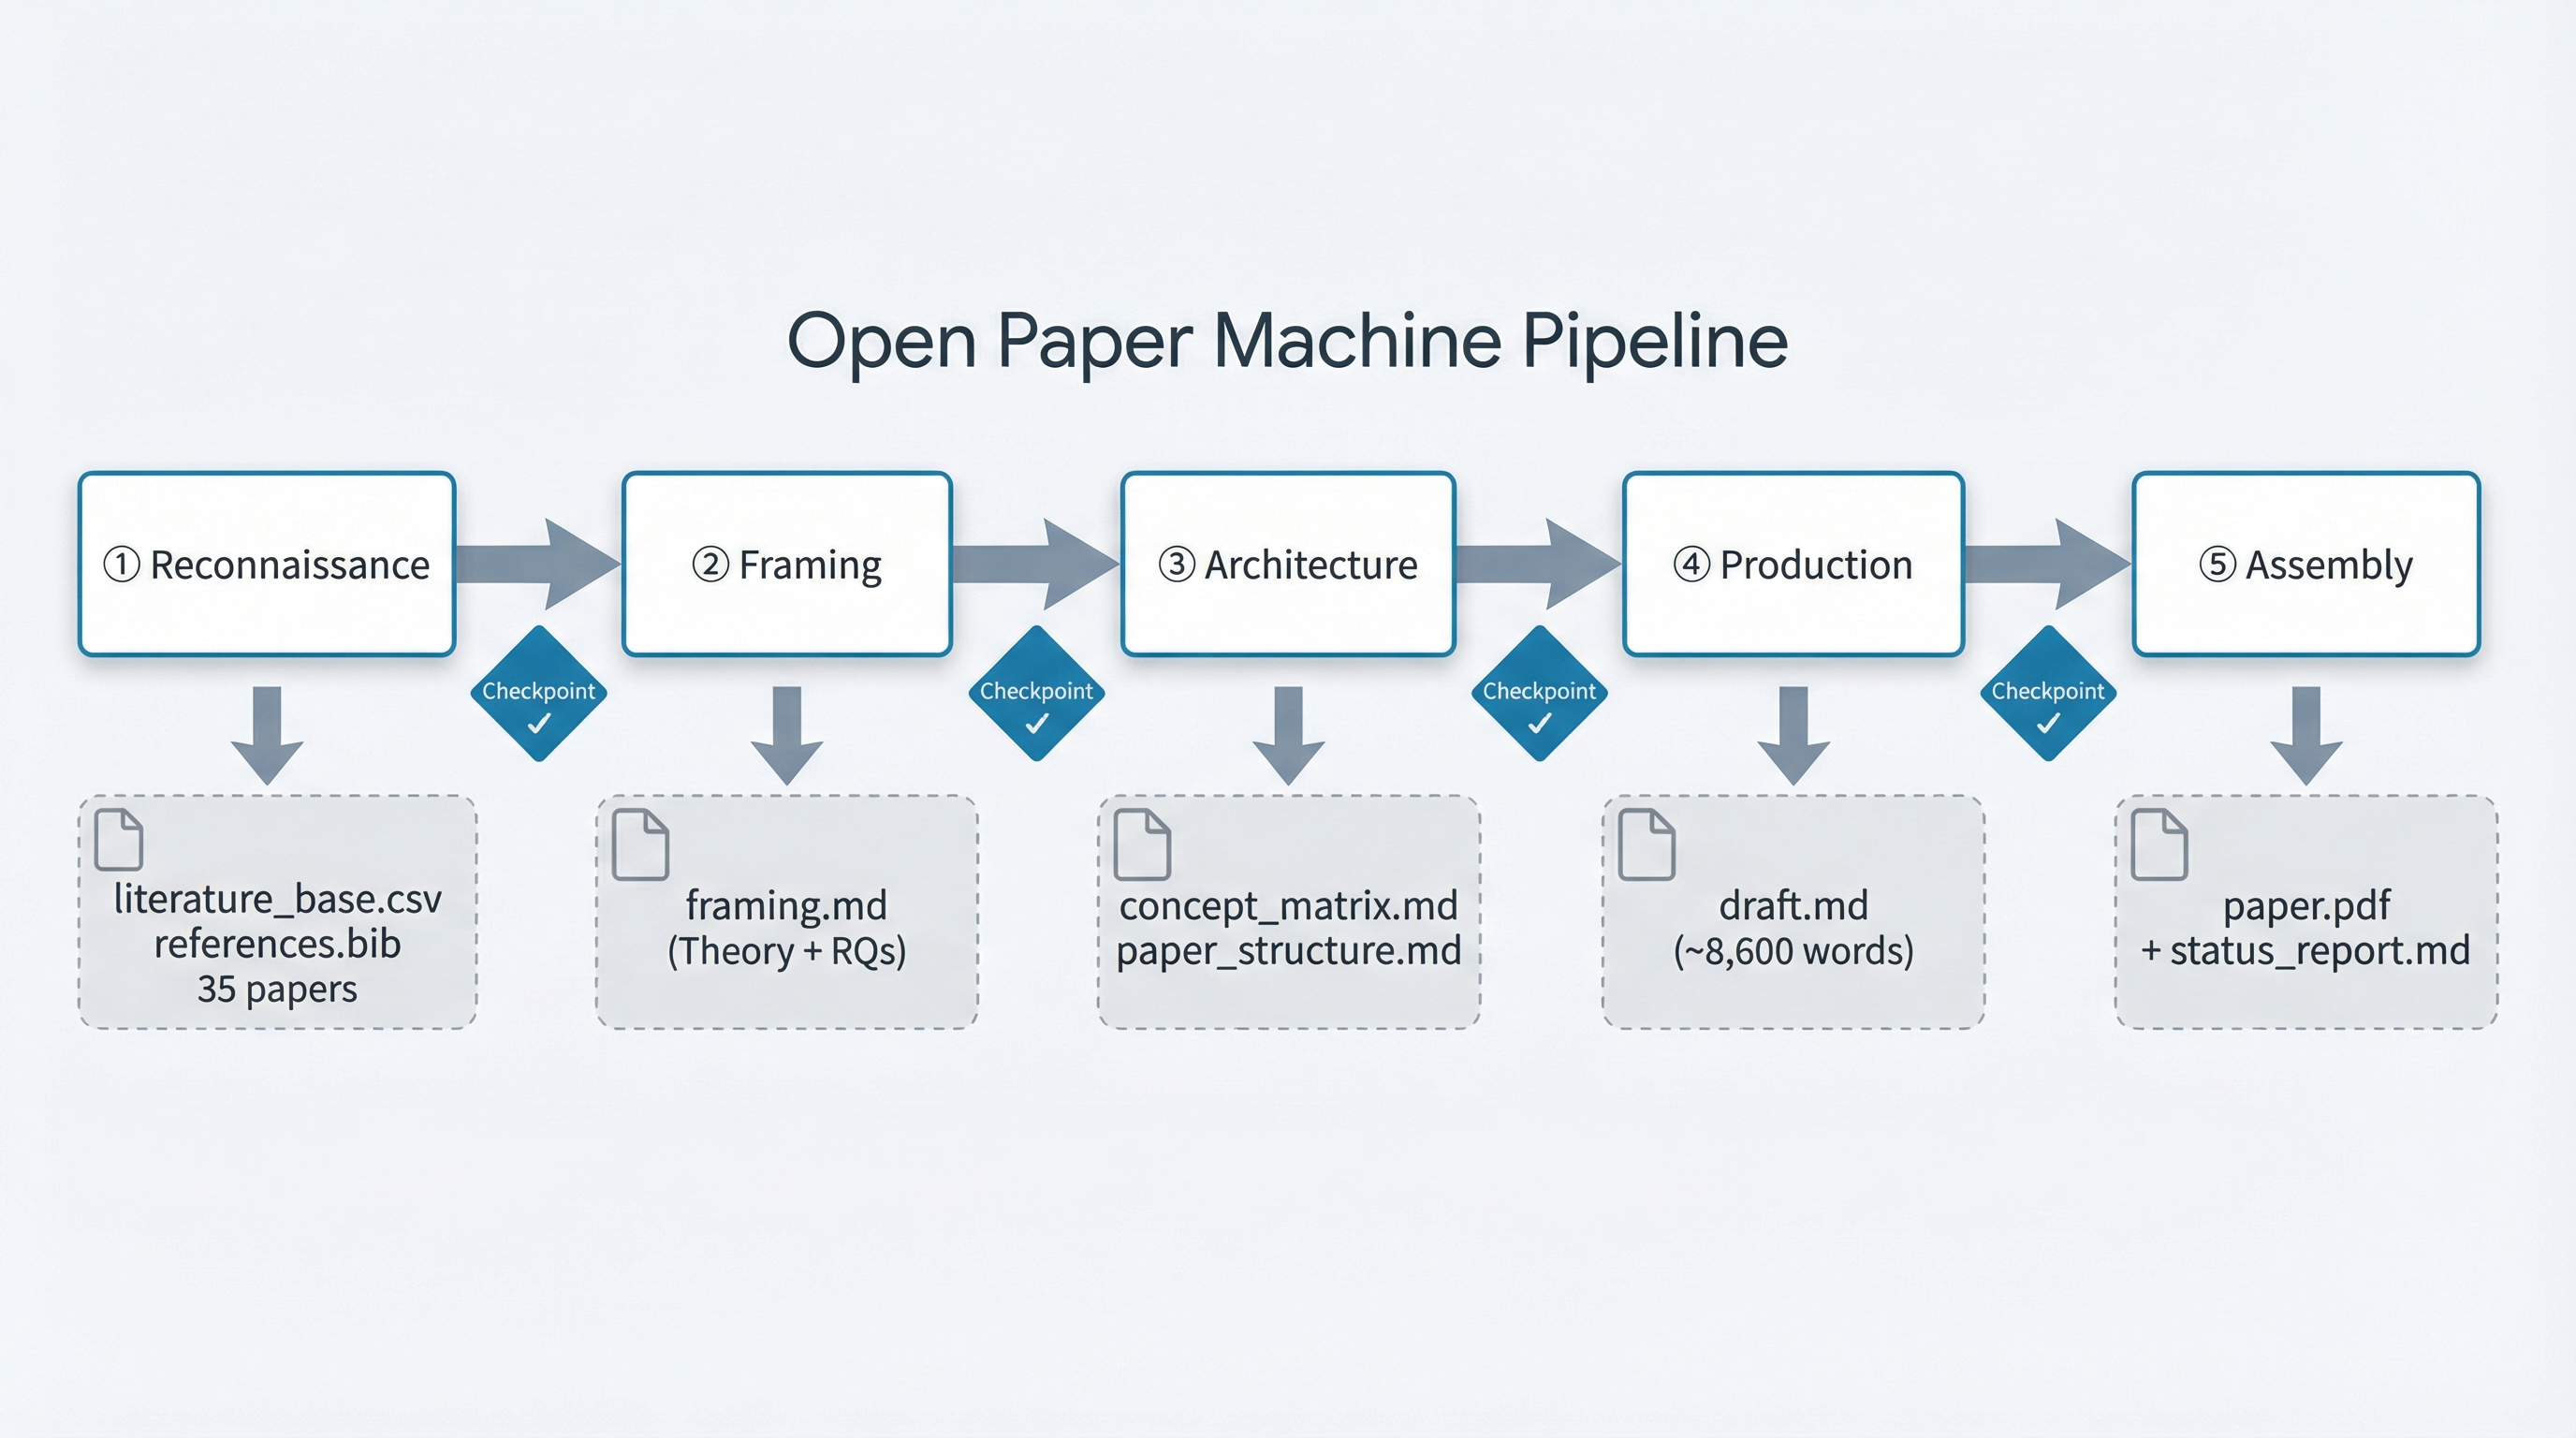
\includegraphics[width=\textwidth]{figures/fig2_pipeline_phases.png}
\caption{The 5-phase research loop: from initialization to final assembly.}
\label{fig:pipeline}
\end{figure}

\begin{table}[htbp]
\centering
\begin{tabular}{lllp{4cm}}
\hline
\textbf{Phase} & \textbf{Primary Agent Role} & \textbf{Key Artifacts} & \textbf{Tools Used} \\
\hline
1. Reconnaissance & Query formulation \& selection & PDF corpus, \texttt{concept\_matrix.csv} & arXiv API, Semantic Scholar API \\
2. Framing & Outline synthesis & \texttt{outline.md} & Local file editing, Bash \\
3. Architecture & Methodological grounding & \texttt{methodology.md} & Search APIs, local retrieval \\
4. Production & Full text drafting & \texttt{draft\_sections/*.md} & Code execution, recursive LLM calls \\
5. Assembly \& Compilation & LaTeX assessment \& formatting & \texttt{paper.tex}, \texttt{figures/} & Bash + PaperBanana (Gemini 3.1 Pro via MCP) \\
\hline
\end{tabular}
\caption{Open Paper Machine operational phases, artifacts, and MCP tools.}
\label{tab:phases}
\end{table}

\begin{figure}[htbp]
\centering
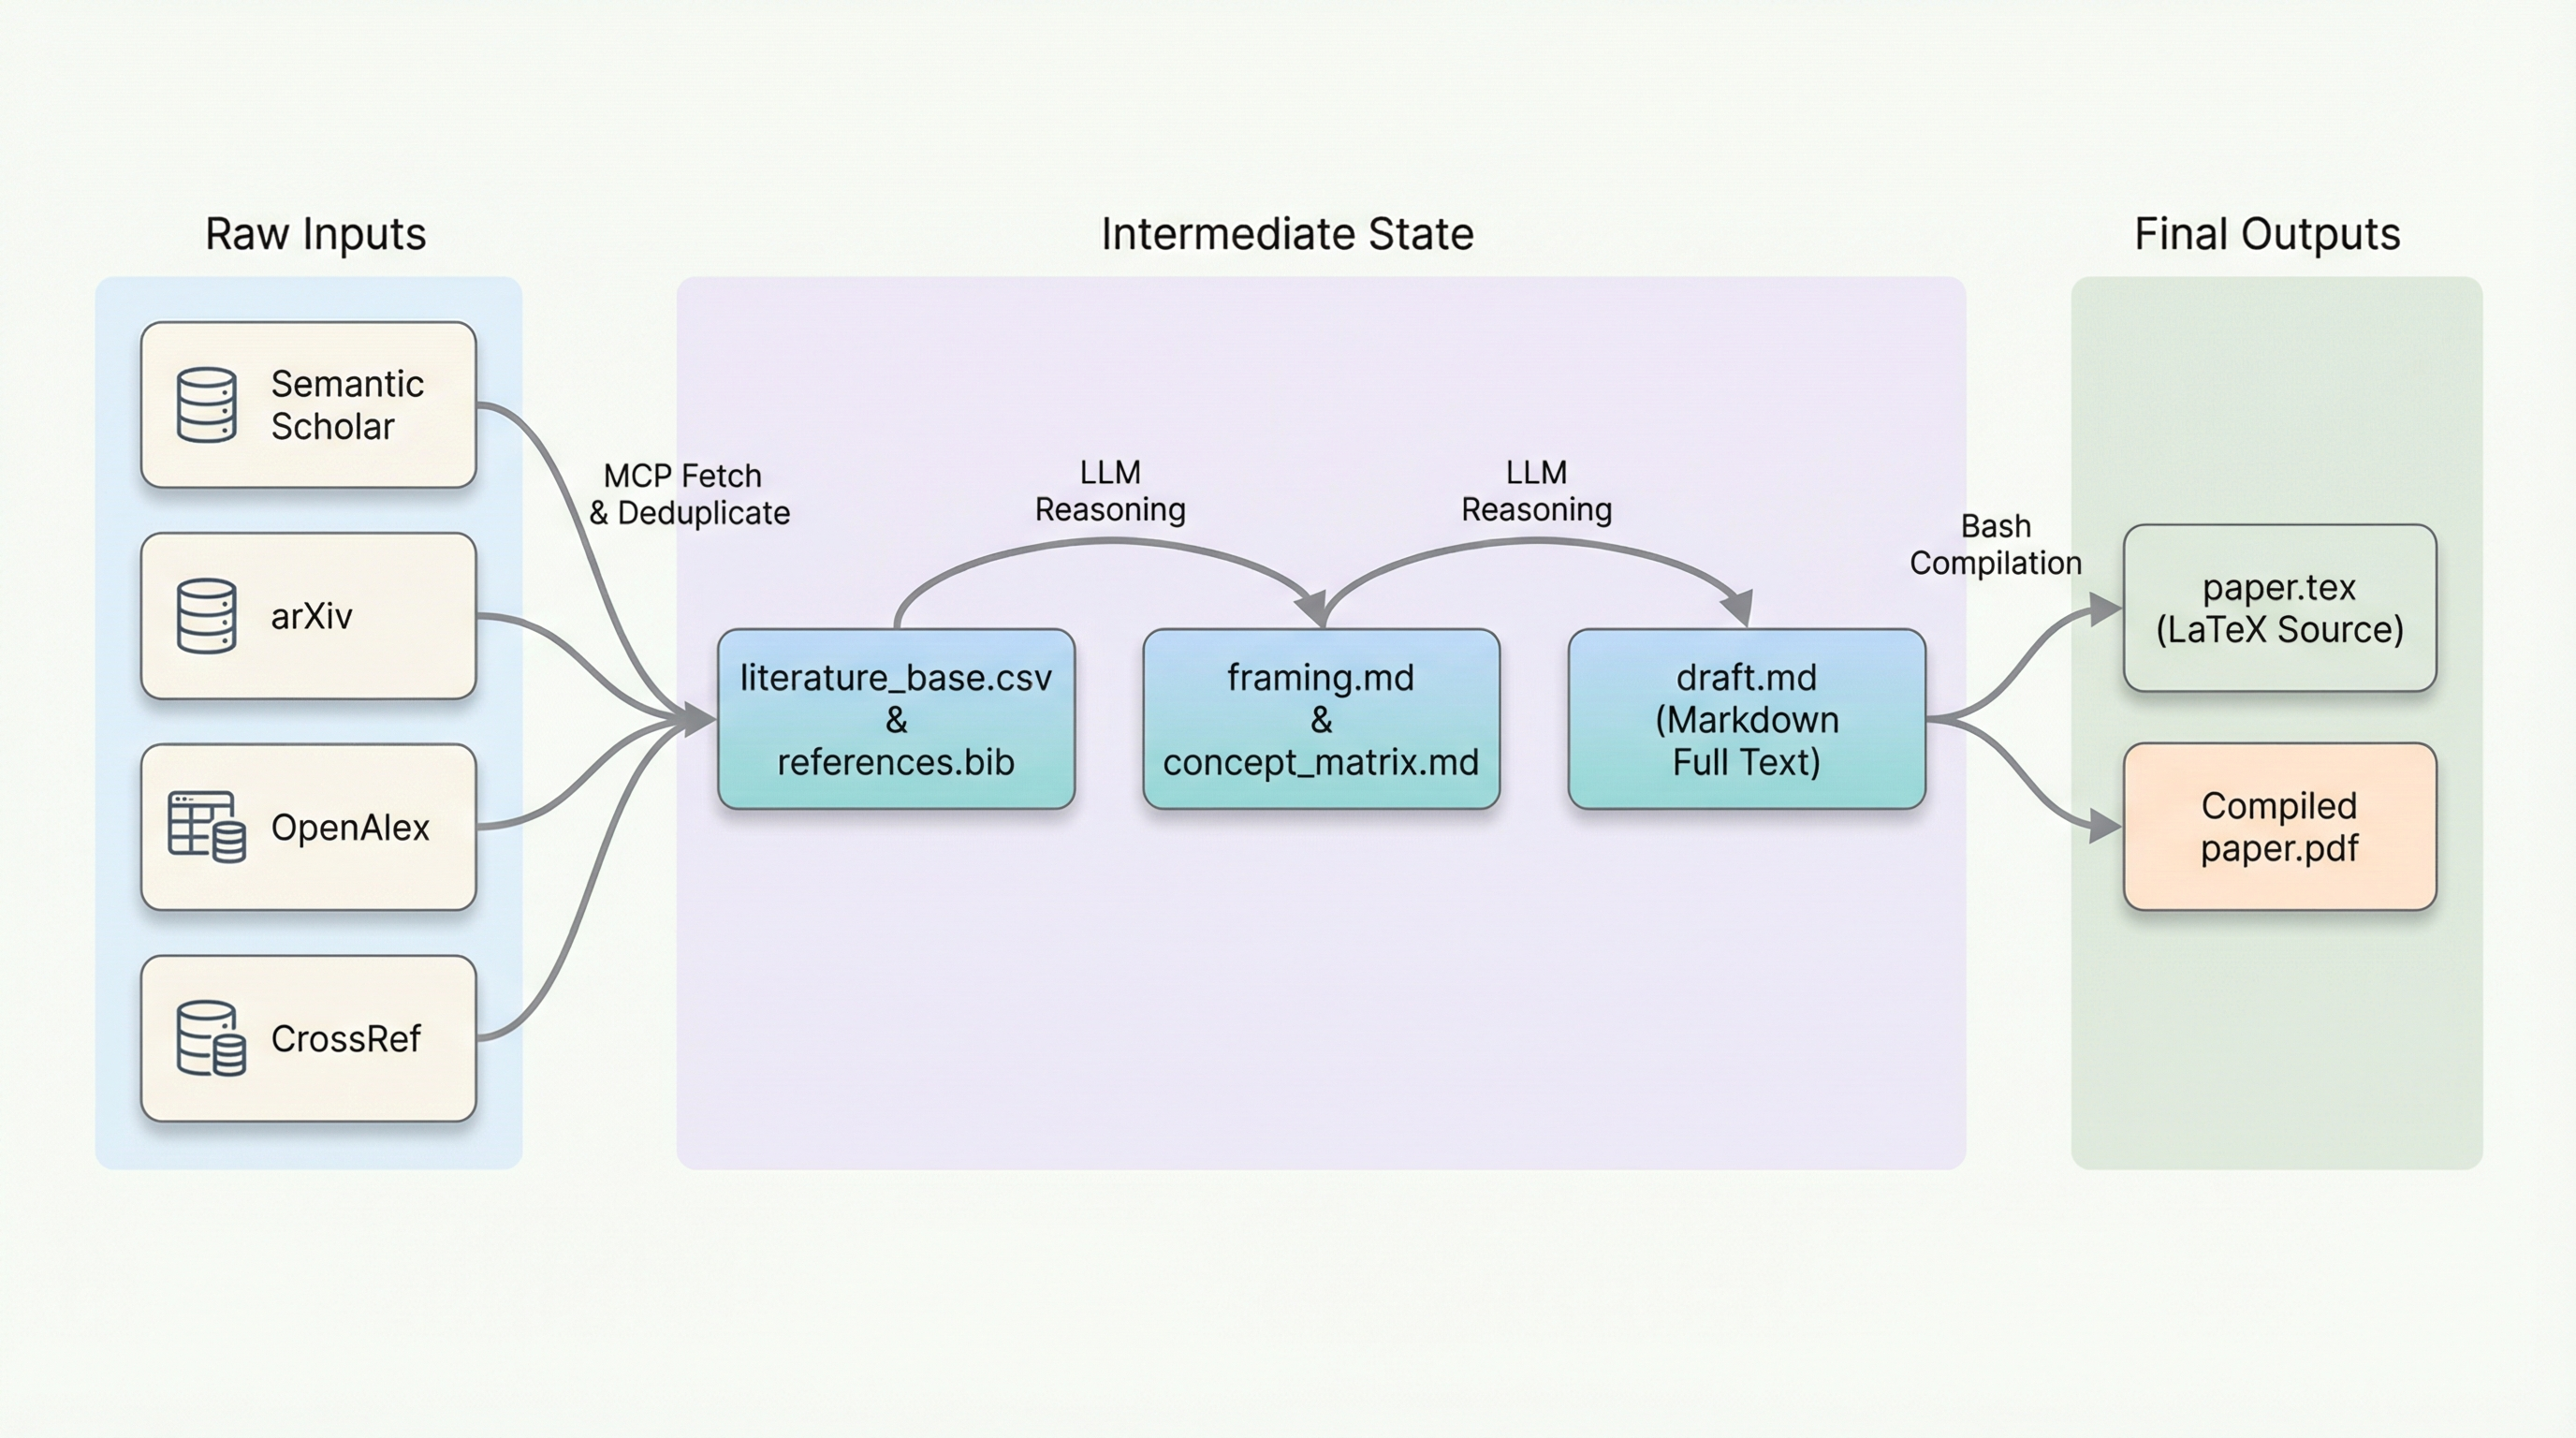
\includegraphics[width=\textwidth]{figures/fig17_artifact_flow.png}
\caption{Artifact flow: detailed data lineage from raw database searches to final assembled LaTeX manuscript.}
\label{fig:artifactflow}
\end{figure}

In designing this system, we explicitly reject the metaphor of the ``AI assistant.'' The
agent requires structured state---scratchpads, task lists, and concept matrices. Tools
without agentic persistence are immediately bounded by context windows.

\begin{figure}[htbp]
\centering
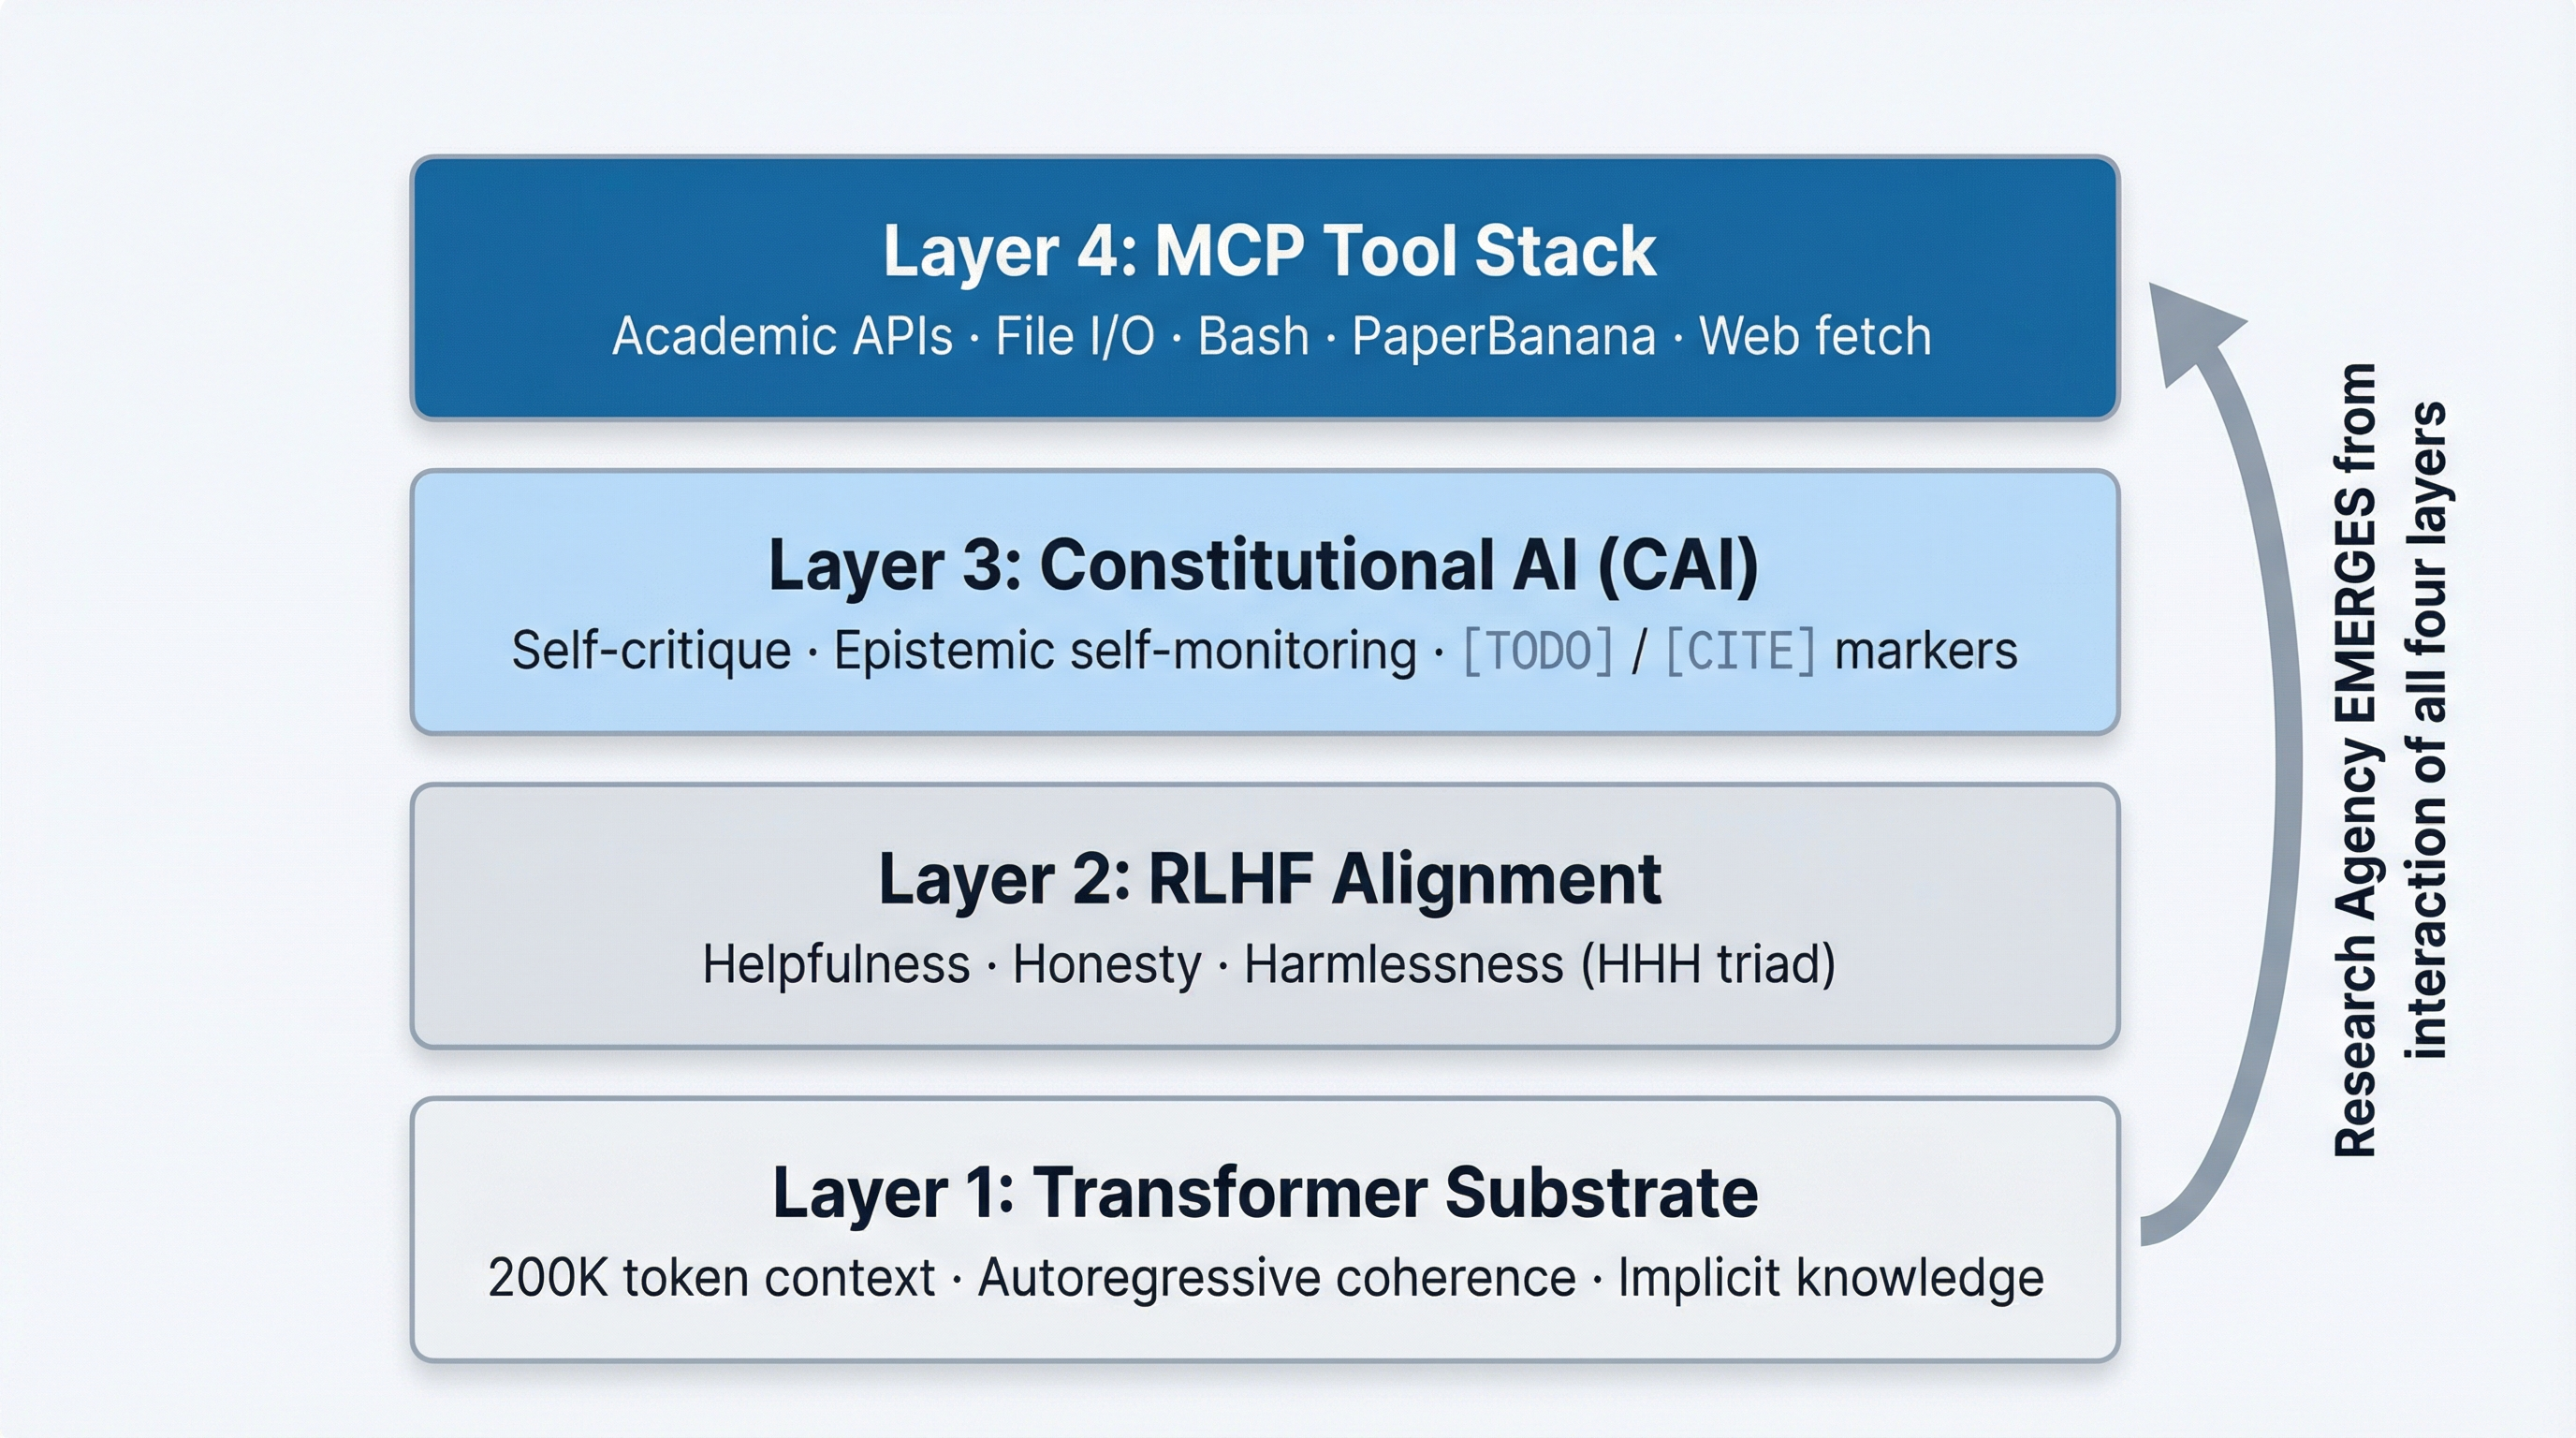
\includegraphics[width=\textwidth]{figures/fig1_architecture_layers.png}
\caption{The four emergent layers of autonomous scientific work: Transformer, Alignment, Agentic Structuring, and The Open Paper Machine.}
\label{fig:architecture}
\end{figure}

\subsection{Tool-Augmented Action (MCP)}

\citet{wang2024survey} characterise tool use as one of three defining features of LLM
agents. The \textbf{Model Context Protocol (MCP)}, introduced by Anthropic in 2024,
standardises the interface for declaring tool capabilities and formatting calls. For the
Open Paper Machine, MCP transforms a text-prediction model into a composable research agent.
It is the ability to read a terminal error, hypothesis why a script crashed, edit the
file, and re-run the command until the PDF compiles.

\begin{figure}[htbp]
\centering

\includegraphics[width=\textwidth]{figures/fig6_capability_matrix.png}
\caption{Capability spectrum of current LLM agents in qualitative IS research, highlighting areas of demonstrated competence versus fundamental limitations.}
\label{fig:capmatrix}
\end{figure}

%% ============================================================
%% SECTION 3: METHODOLOGY
%% ============================================================
\section{Methodology}
\label{sec:methodology}

\subsection{Design Science with a Reflexive Twist}

This paper adopts a reflexive design science orientation \citep{hevner2004design}. The
artifact is the Open Paper Machine and its output---this paper plus all intermediate
artifacts. We evaluate against two objectives: \emph{academic quality} and \emph{evidential
value}.

\subsection{The Pipeline as Data}

\subsection{Quality Criteria}

Four criteria, adapted from \citet{lincoln1985naturalistic}: credibility, transferability,
confirmability, and reflexivity. All intermediate artifacts are archived---prompts, tool
calls, files, generation sequence.

\subsection{Ethics: The Authorship Question}

We adopt the \emph{orchestrator model}: the human (Blask) is the accountable author who
designed the task, evaluated outputs, and approved the paper. Claude is disclosed as the
text generator---analogous to a research assistant who contributes substantially but does
not receive authorship credit \citep{dwivedi2023chatgpt}.

%% ============================================================
%% SECTION 4: ARCHITECTURE
%% ============================================================
\section{Architecture: Four Layers of the Open Paper Machine}
\label{sec:architecture}

The agent loop follows ReAct \citep{yao2022react}: Reason--Act--Observe cycles. The
critical property is \emph{composability}: tools combine in any order, with results from
one informing the next.

\subsection{Emergence: The Whole Exceeds the Sum}

The four layers interact, not sum. Research agency \emph{emerges} from this interaction:
transformer (extended reasoning) + RLHF (epistemic dispositions) + CAI (self-monitoring)
+ Tools (external reach). Remove any component and the system degrades.

%% ============================================================
%% SECTION 5: CAPABILITIES AND FAILURE MODES
%% ============================================================
\section{Capabilities and Failure Modes}
\label{sec:capabilities}

Four fundamental failure modes:

\begin{enumerate}
\item \textbf{Training cutoff.} Parametric knowledge frozen at training time.
\item \textbf{Hallucination.} LLMs generate plausible-sounding but factually incorrect
content \citep{zhang2025hallucination}. All citations require human verification.
\item \textbf{Overconfident synthesis.} May elide contradictions or null results.
\item \textbf{No primary data.} Cannot conduct experiments, surveys, or fieldwork.
\end{enumerate}

\subsection{Comparison with Prior Systems}

\begin{figure}[htbp]
\centering

\includegraphics[width=\textwidth]{figures/fig9_system_comparison.png}
\caption{Comparison of tool-augmented search flows. Traditional flows rely on human curation; the Open Paper Machine automates retrieval, assessment, and synthesis.}
\label{fig:syscomp}
\end{figure}

The Open Paper Machine compresses the first three phases (literature, framing, design) to
$\sim$40 minutes. This implies a \emph{skill shift}: less valued are Boolean search
construction and manual abstract screening; more valued are formulating precise research
briefs and evaluating AI synthesis critically.

\subsection{Authorship and Accountability}

We propose the \textbf{orchestrator model}: the human who formulates the task, evaluates
outputs, and accepts accountability is the author. The AI system is disclosed as a
generator. The distinction is accountability, not contribution.

\subsection{Peer Review Under Pressure}

Rather than attempting to train a model that does not hallucinate, we need protocols that
assume hallucinations will occur and catch them through structural guarantees.

\begin{figure}[htbp]
\centering
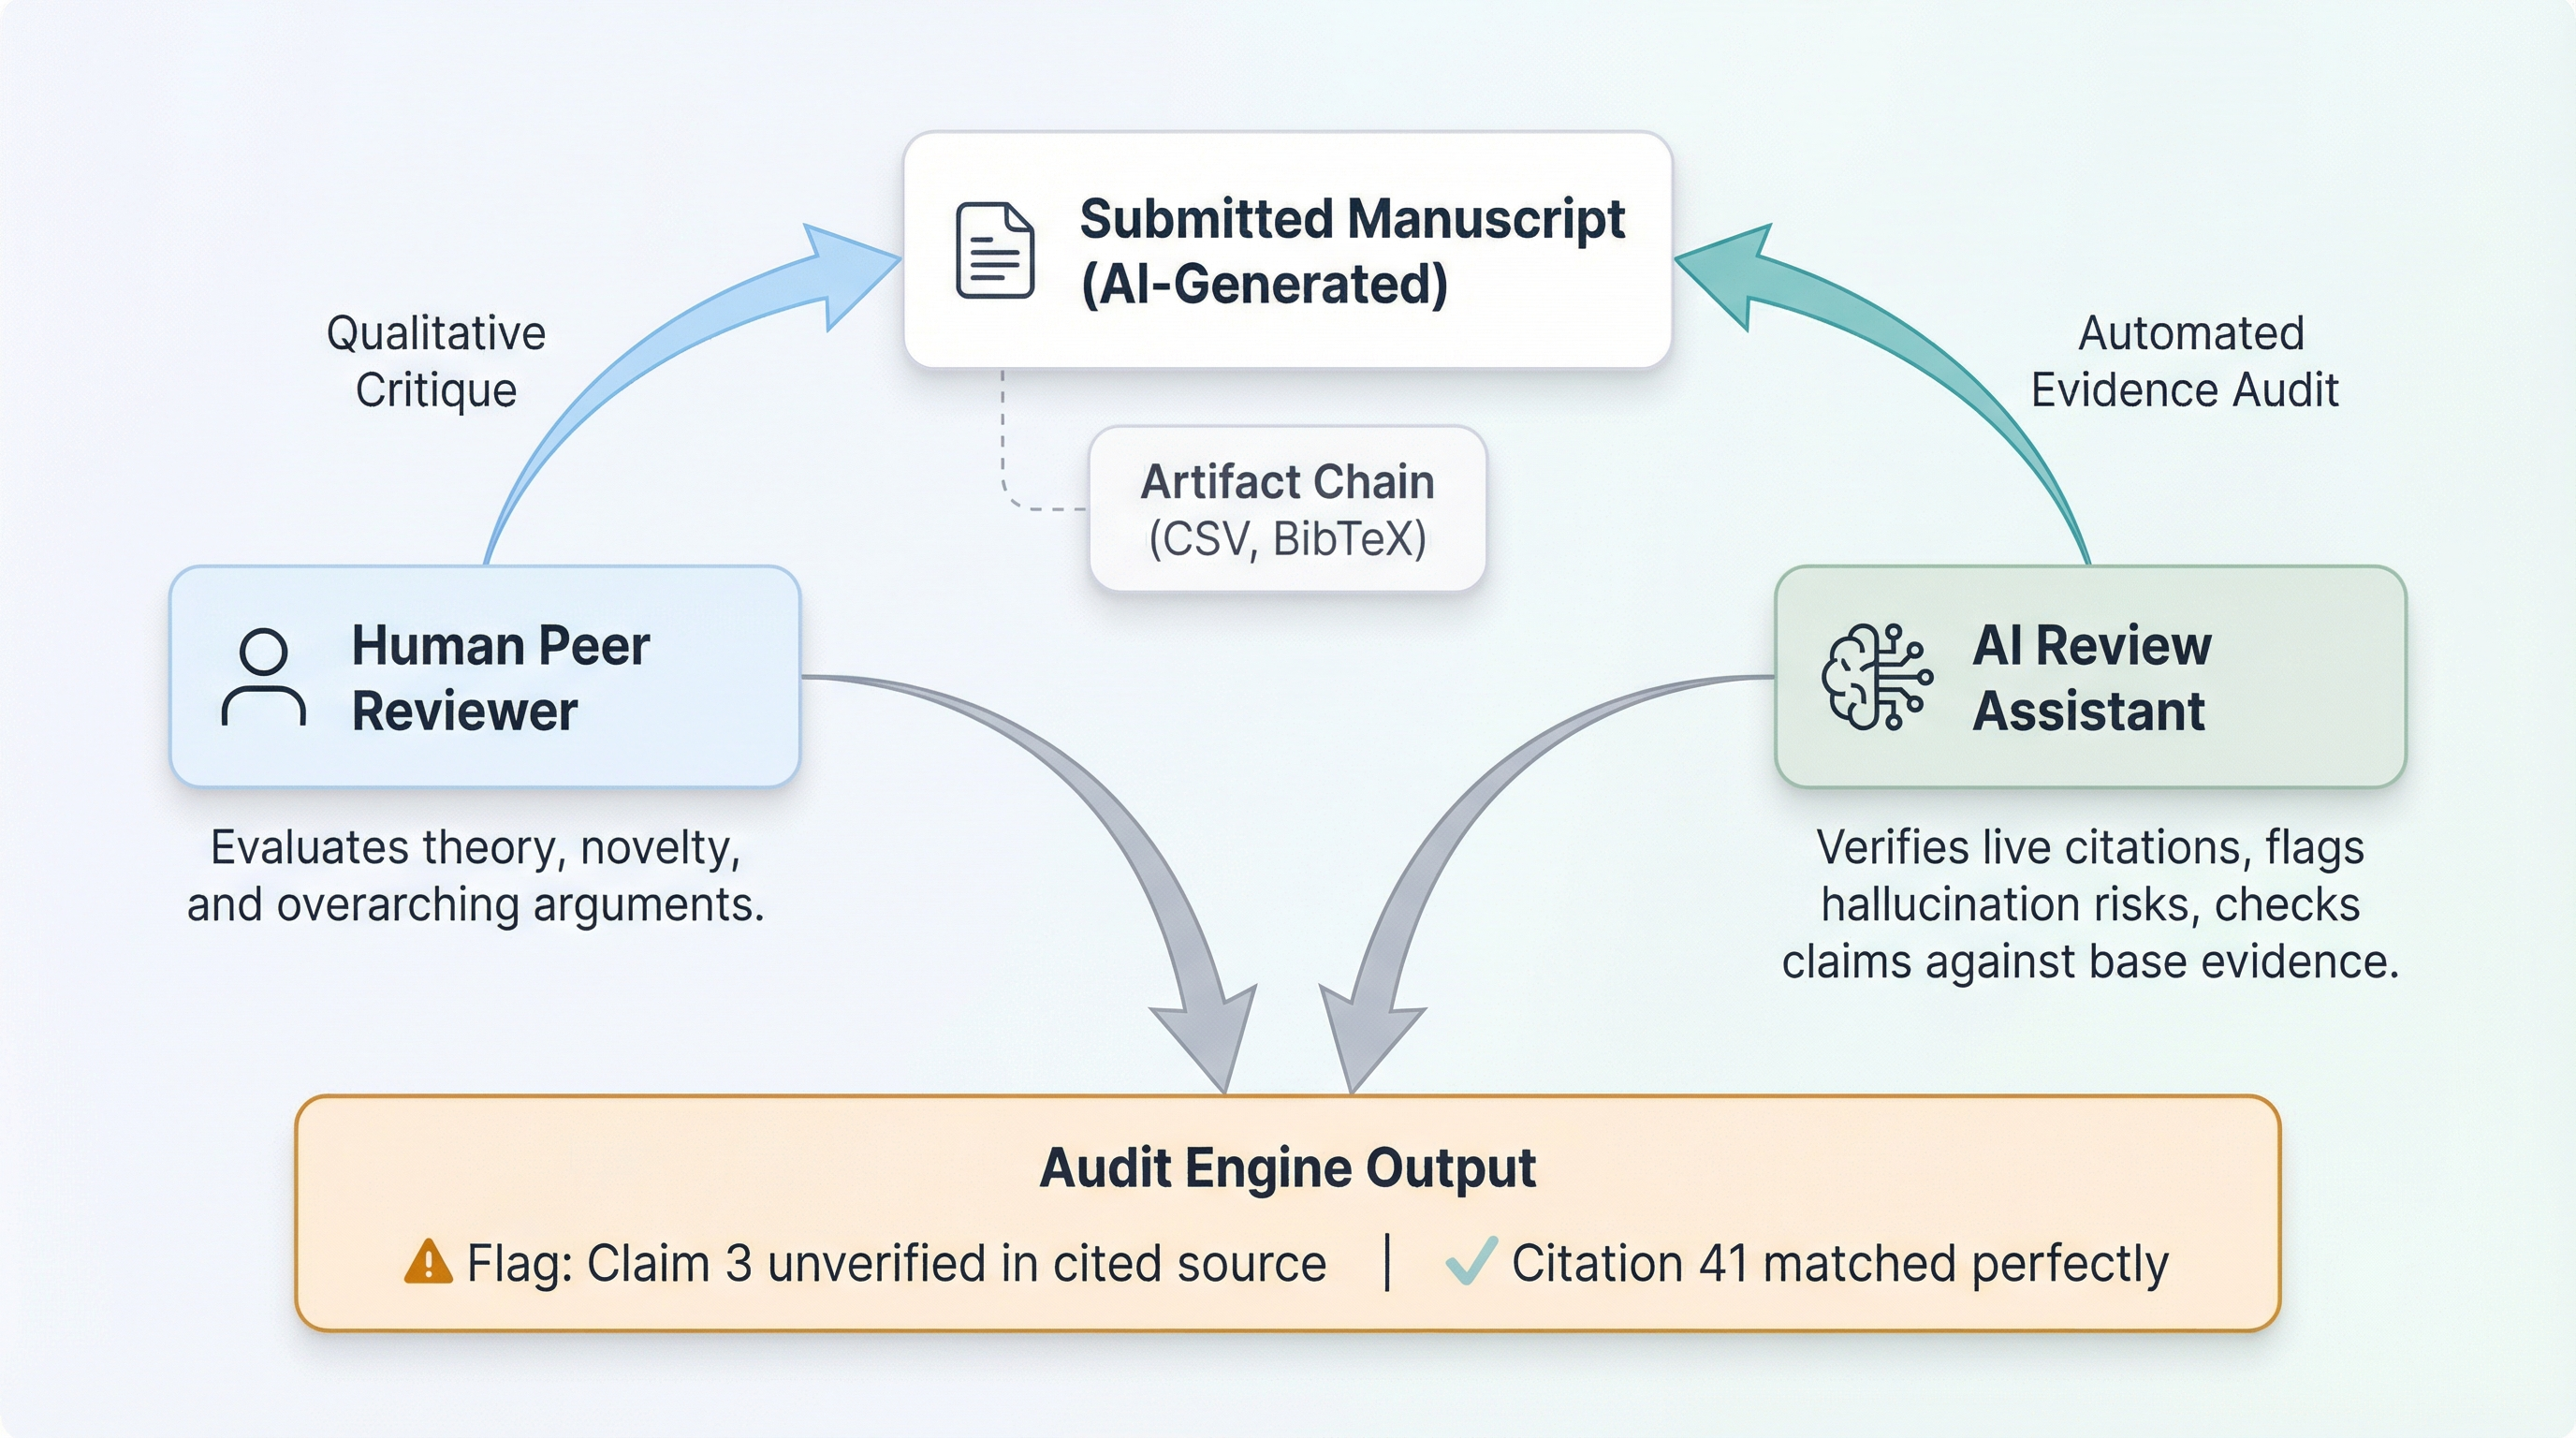
\includegraphics[width=\textwidth]{figures/fig18_peer_review_loop.png}
\caption{AI-augmented peer review system tracking hallucination risks and claim evidence.}
\label{fig:peerreview}
\end{figure}

\subsection{Reconfiguring the Researcher Role}

AI-augmented peer review could check citations against live databases, flag hallucinated
references, and identify claims exceeding their evidence. The pipeline artifacts
(CSV, BibTeX, concept matrix) model how AI-generated research might be made auditable.


This conclusion was written by the system it describes. The model cannot step outside itself.
Its acknowledgment of limitations is a product of Constitutional AI training---and may
therefore be systematically incomplete in ways the model cannot detect.

What this paper demonstrates is not that AI has achieved scientific understanding. It
demonstrates that the boundary between human and AI epistemic contribution is becoming
productively blurry---and that blur demands serious theoretical and institutional attention.

\vspace{1em}\hrule\vspace{0.5em}

\noindent\emph{This paper was produced by Claude Opus 4.6 (Anthropic PBC) under
orchestration by Tobias-Benedikt Blask (Harz University of Applied Sciences). All pipeline
artifacts are available for audit. Code: \url{https://github.com/tobiasblask/open-paper-machine}}

%% ============================================================
%% BIBLIOGRAPHY
%% ============================================================
\bibliographystyle{plainnat}
\bibliography{../references}

\end{document}
